\chapter{توضیح مختصری بر الگوریتم}

در فصل \ref{ch:rl} در مورد مفاهیم \w{rl} بحث شد. مهمترین مفاهیم عبارتند از:
\begin{multicols}{3}
\begin{enumerate}
	\item \w{env} \item \w{agent} \item \w{env state} \item \w{agent state} \item \w{reward} \item \w{observ} 
\end{enumerate}
\end{multicols}

هدف در این پروژه این بود که یک \w{autocar} با استفاده از الگوریتم های \w{rl} ساخته شود. جزییات تئوری الگوریتم و جزییات فنی پروژه به ترتیب در بخش های 
\ref{ch:rl}
و
\ref{ch:fani}
آورده شده‌اند.
در این بخش به شبیه سازی و جزییات کار و تعریف پارامتر های این پروژه برداخته می‌شود.

\section{معرفی محیط شبیه سازی}

در ابتدا محیط شبیه سازی را معرفی می‌کنیم. جزییات فنی این محیط در \ref{ch:fani} و همچنین نحوه راه‌اندازی آن در بخش \ref{ch:resault|sec:launch} به‌صورت کامل مورد بحث قرار گرفته است. اگر آن محیط را باز کنید محیط مانند شکل 
\ref{fig:obs-1}
باز خواهد شد. این محیط دو آبجکت مهم دارد؛
\begin{alphinline}
	\item ماشین(اتومبیل)
	\item جاده
\end{alphinline}
(شکل \ref{fig:road-car-models}) 



\begin{figure}
	\centering
	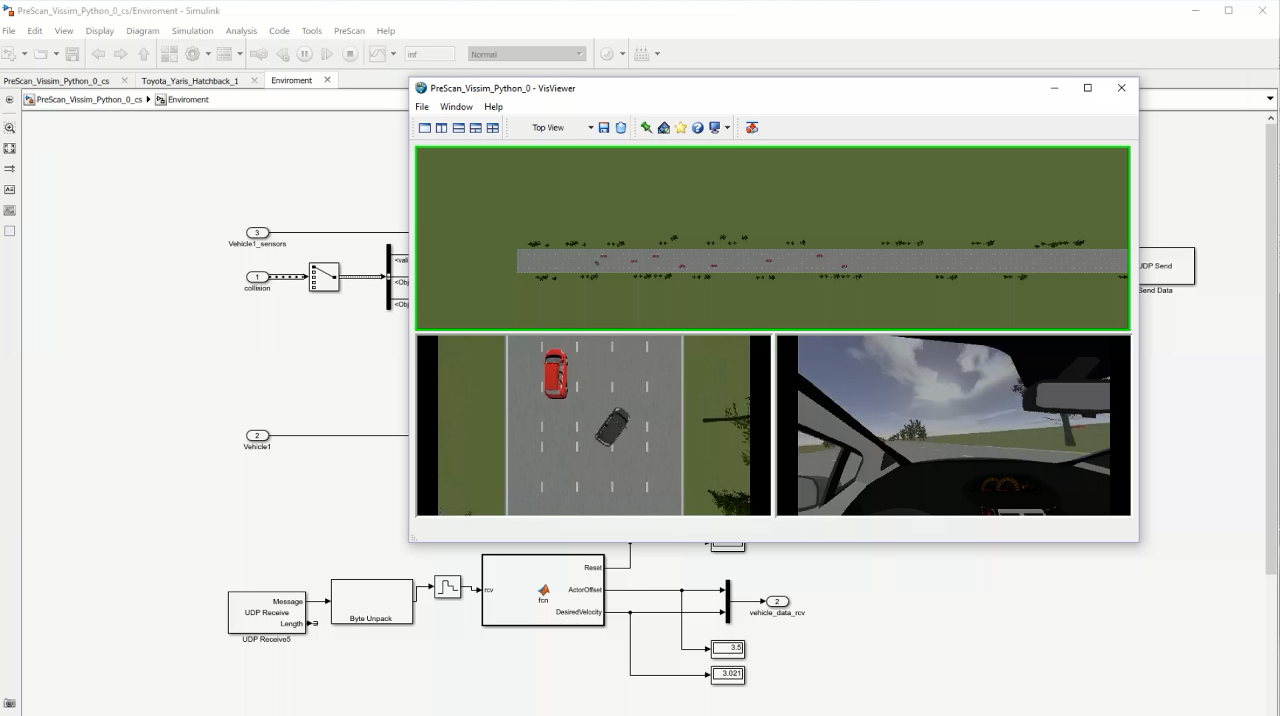
\includegraphics[width=0.7\linewidth]{Figures/OBS/1}
	\caption{محیط شبیه سازی}
	\label{fig:obs-1}
\end{figure}


%HERE
\begin{figure}
	\centering
	\def\localheight{2cm}
	\subfigure[]{%
		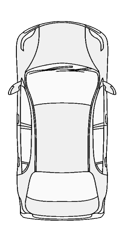
\includegraphics[height=\localheight]{Figures/rzbinary/agent}
		\label{subfig:model-car}
	}
	\hspace*{0.5cm} % space between two figures
	\subfigure[]{%
		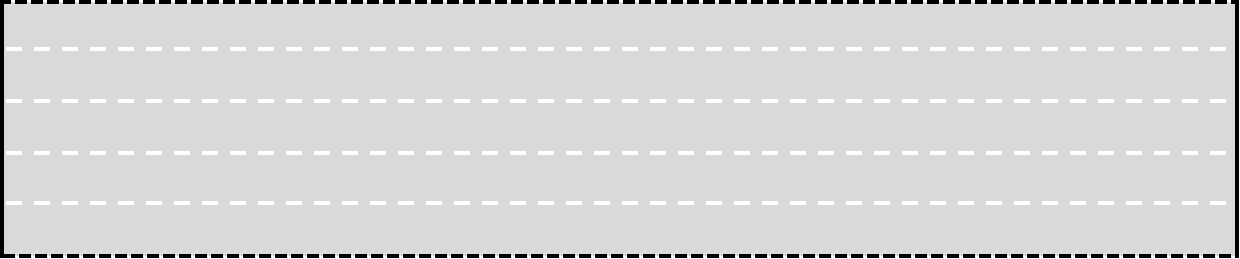
\includegraphics[height=\localheight]{Figures/rzbinary/road}
		\label{subfig:model-road}
	}
	\caption[]{%
	}
	\label{fig:road-car-models}
\end{figure}


چیزی که اهمیت دارد اندازه ها و نحوه تعریف محدوده هاست. شکل \ref{fig:road-car-total} اندازه‌ها و محدوده ها را مشخص کرده است. 
شکل \ref{subfig:road-car-redbox-w} نشان می‌دهد که این محدوده ها کاملا برروی یک دیگر منطبق نیستند. دلیل اصلی این موضوع عدم اهمیت تطبیق دقیق این دو می‌باشد. در بخشی که پشت ماشین قرار دارد این محدوده از $-4$ (کمی بیشتر از اندازه عرض لاین ها) شروع می‌شود. زیرا نیازی نیست بیشتر از این مقدار ماشین مورد بررسی به عقب برود تا متوجه شویم اشتباه در حال رفتن است. درحقیقت این مورد کمک می‌کند تا تعداد \w{step} ها را در هر \w{episode} اشتباه کاهش یابد. بخش های کناری نیز از $-11$ تا $+11$ محدود شده‌اند (بیشتر از عرض خود جاده) تا اگر نوسانی یافت به ماشین این اجازه داده شود تا به مسیر اصلب برگردد. 



\begin{note}
	ماشین در مبدا صفحه قرار دارد. از این رو اعداد منفی نسبت به همین ماشین نیز سنحیده می‌شوند.
\end{note}



\begin{figure}[b!]
	\centering
%	\def\localdata{}
	\subfigure[]{%
		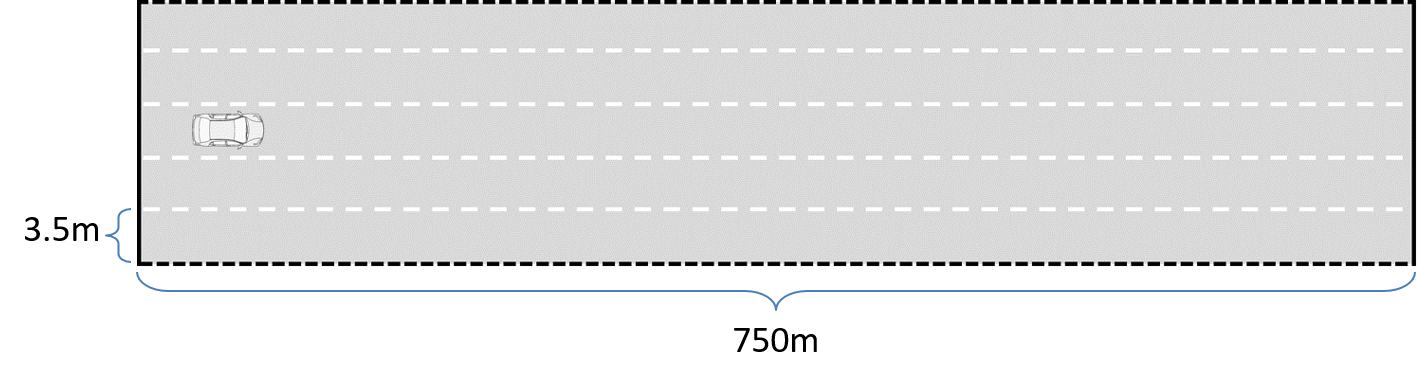
\includegraphics[width=0.7\linewidth]{Figures/rzbinary/road-car-wh}
		\label{subfig:road-car-wh}
	}
	%  	\hspace*{1.5cm} % space between two figures
	\subfigure[]{%
		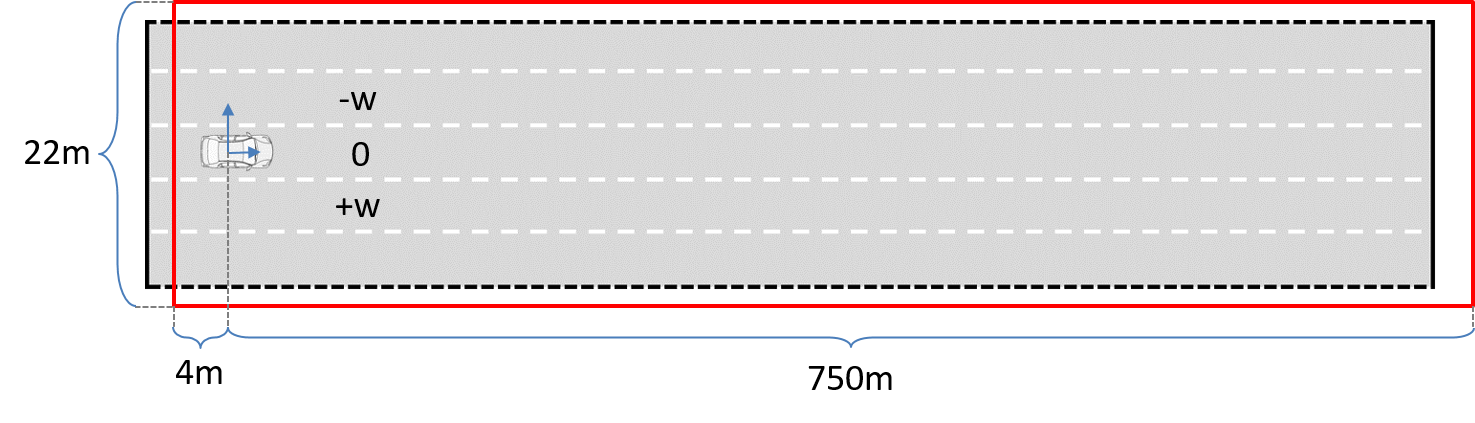
\includegraphics[width=0.7\linewidth]{Figures/rzbinary/road-car-redbox+-w}
		\label{subfig:road-car-redbox-w}
	}
	\caption[]{%
	}
	\label{fig:road-car-total}
\end{figure}

3 مقدار \lr{+w} ، \lr{-w} و \lr{0} که در شکل \ref{subfig:road-car-redbox-w} بر روی جاده نوشته شده است در حقیقت مرتبط با بحث فنی ماجرا می‌باشد اما مفهوم آن این است که \w{agent} مورد بررسی می‌تواند این سه لاین را به عنوان \w{action} اختیار کند. در حقیقت می‌توان آن‌ها را به عنوان اسم برای هر لاین در نظر گرفت. در مورد \w{action} بیشتر صحبت خواهد شد.

\begin{note}
	راه‌اندازی این محیط کمی دردسر خواهد داشت از این‌رو نیاز است پیش از راه‌اندازی بخش \ref{ch:resault|sec:launch} به‌طور دقیق مطالعه شود.
\end{note}






\section{تعریف کردن پارامتر های \ws{rl}}
قبل از بررسی پارامتر های ‌\w{rl} مناسب است که شکل نهایی این الگوریتم همین ابتدا بررسی شود.
\footnote{منظور از پارامتر های \w{rl} پارامتر هایی مانند تعیین \w{reward} و \w{state} می‌باشد.
}
در این پروژه دو الگوریتم \gls{a:dqn} و \gls{a:a2c} بهتر از سایر الگوریتم ها عمل کردند اما در نهایت با توجه به آزمایش‌ها و ملاحظاتی که انجام شد، الگورینم \gls{a:dqn} از لحاظ سرعت همگرایی بهتر از الگوریتم \gls{a:a2c} پاسخ داد. بنابراین صرفا برروی این الگوریتم بحث خواهد شد.




\code[python, label={code:dqn.py}]{dqn-train.py}


این کد بخش \w{train} را نشان می‌دهد. بخش \w{test} در تمامی الگوریتم ها مشابه یک دیگر است و از جایی که مدل تعریف می‌شود (در اینجا خط 18) شروع خواهد شد. 

بخش \w{test} در تمامی الگوریتم ها کد زیر است.

\code{alg-test.py}

از روی چند خط آغازین کد
\hyperref[code:dqn.py]{\gls{a:dqn}}
می‌توان دریافت که این کد با استفاده از \lr{gym}\cite{git/gym} و \lr{stable-baseline}\cite{stable-baselines} نوشته شده است.

بخش مهم بعدی متغیری از جنس دیکشنری به نام \texttt{env\_dict} است. این متغیر برای ساختن متغیر \texttt{env} در دستور 
\lr{\texttt{env = gym.make(**env\_dict)}} 
به‌کار می‌رود.
\RTLfootnote{متغیر \texttt{env} در حقیقت نقش \w{env} را در الگوریتم دارد.}
 توضیح این متغیر و اجزای آن در جدول \ref{tab:env-dict} آمده است.
 
\begin{table}\tableset{
\begin{tabular}{|C{0.25\linewidth}|p{0.7\linewidth}|}
	\hline\rowcolor{lightgray}
	متغیر & توضیحات
	\\\hline
	\texttt{id} & در این پروژه این متغیر دو حالت بیشتر ندارد که هردو از جنس رشته هستند. اگر این کد با استفاده از \w{matlabengine} استفاده شود، \lr{\texttt{'prescan-v0'}} 
	خواهد بود و اگر از \w{matlabengine} استفاده نشده باشد مقدار آن 
	\lr{\texttt{'prescan-without-matlabengine-v0'}} 
	خواهد بود. 
	
	این متغیر مقدار پیش‌فرض ندارد.
	 \\\hline
	\texttt{verbose} & این متغیر که از جنس بولین می‌باشد، در صورتی که یک باشد اطلاعات جامعی را در هر \w{step} 
	را چاپ می‌کند. علاوه برآن اطلاعات آماری \w{reward}های بدست‌آمده در پایان هر \w{episode} را نیز چاپ می‌کند. به‌طور کلی اجازه گزارش دادن و ندادن اطلاعات درونی الگوریتم توسط این متغیر کنترل می‌شود.
	 \\\hline
	\texttt{host} & \\\hline
	\texttt{delay} & \\\hline
	\texttt{nget} & \\\hline
	\texttt{experimant\_name} & \\\hline
	\texttt{close\_window} & \\\hline
\end{tabular}}
\caption{}
\label{tab:env-dict}
\end{table}

